 \section{Methodology}
\label{sec:Method}
Prior to proposing more specific guidelines for developing a tactic search engine, we conducted an extensive study of architectural decisions and their implementations in 40 performance centric, safety critical dependable systems\cite{FSE2012}.

\subsection{Goals}
Current research lacks insight into the implementation of tactics. Revealing low-level and non-abstract issues in developing architectural tactics can help shape the foundation of a tactic search engine.

 \subsection{Research Question}
Our study is focused on the following research question: \emph{What are the implementation characteristics of architectural tactics that are reflected in the source code?}



\subsection{Project Selection}
The following process was used to select a set of open source projects for this study.

\begin{itemize}

   \setlength{\itemsep}{0pt} %Cut down on spacing for the different items in the list
   \setlength{\parskip}{0pt} %Cut down on spacing for the different items in the list
   \setlength{\parsep}{0pt}  %Cut down on spacing for the different items in the list

\item \textit{Selection through Code Search:} The source code search engine \textit{Koders} was used to locate projects which have implemented a set of predefined architectural tactics. The search query for each tactic is composed of keywords used in the libraries that the architect has previously used to implement the tactics. The results have been peer reviewed to ensure that each project has implemented the architectural tactic.


\item \textit{Selection by Meta-Data:} Project-related documents, such as design documents and online forums were searched for references and pointers to architectural tactics. This search was followed by a detailed source code review to ensure that each identified project has the tactics implemented.
\end{itemize}

We have identified 40 open source projects using this process. The projects are elicited from different application domains, with diverse sizes, and developed using different programming languages. This dataset includes projects which are comparable to industrial applications including Chromium, Apache Hadoop, Ofbiz and Hive.

\subsection{Study: Learning from the Trenches}
For each of the examined projects we identified architecturally significant requirements, architectural tactics used to address them, and source files used to implement tactics. For all identified tactics, a peer-code review was conducted to extract code snippets implementing the tactics. This was followed by a manual reverse engineering process where our team members utilized Sparx Enterprise Architect\footnote{\url{http://www.sparxsystems.com/products/ea/downloads.html}} reverse engineering features to draw a class diagram for each instance of the tactic. In this study, two code reviewers who are experienced in software architecture were asked to document their observations of tactic implementations and formulate the challenges that impacts the development of a tactic search engine.

%The following section presents the results of this study.
\section{Qualitative Study}
\label{sec:SeenUnSeen}
As a result of this study we observed five issues related to our research questions that can also significantly influence development of a practical tactic search engine:

\subsection{No Single Solution}
There is no single way to address quality requirements and also no single way to implement an architectural tactic. System tactics may be implemented entirely differently from one system to another. This divergence is due to the differences in the context and constraints of each project. For example, we reviewed the implementation of the \emph{Heartbeat} tactic for reliability concerns in 20 different software systems. We observed the Heartbeat tactic being implemented using (i) direct communication between the emitter and receiver roles found in~\emph{(Chat3 and Smartfrog systems)}, (ii) the Observer pattern where the receiver is registered as a listener to the emitter found in the \emph{Amalgam system}, (iii) the Decorator pattern in which the Heartbeat functionality was added as a wrapper to a core service found in~\emph{(Rossume} and~\emph{jworkosgi systems)}, and finally (iv) numerous proprietary implementations which did not follow any documented designs.

\textit{Therefore a tactic-search engine can not primarily rely on structural dependencies as a means of learning the best tactic implementation.}

\begin{figure}[!htb]
\centering

\subfigure[HeartBeat with configuration files]{
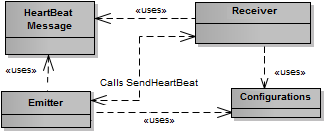
\includegraphics[width=.4\textwidth]{img/HB1.png}
\label{fig:HB1}
}

\subfigure[Observer design pattern to implement the tactic]{
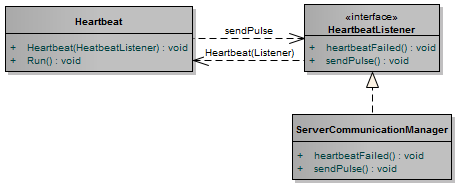
\includegraphics[scale=0.45]{img/HB2.png}
\label{fig:HB2}
}
\subfigure[Decorator design pattern to implement the tactic]{
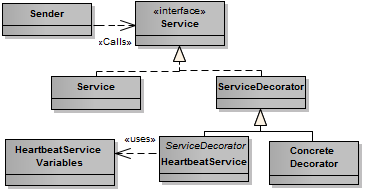
\includegraphics[width=.45\textwidth]{img/HB3.png}
\label{fig:HB3}
}
\label{fig:HBall}
\caption[Heartbeat tactic in different systems]{Hadoop : \subref{fig:HB1}Hadoop, Chat3, smartfrog \subref{fig:HB2}Amalgam System \subref{fig:HB3}Thera, JSRB, Rossume Systems}
\end{figure}

\begin{figure}[tbph]
\centering
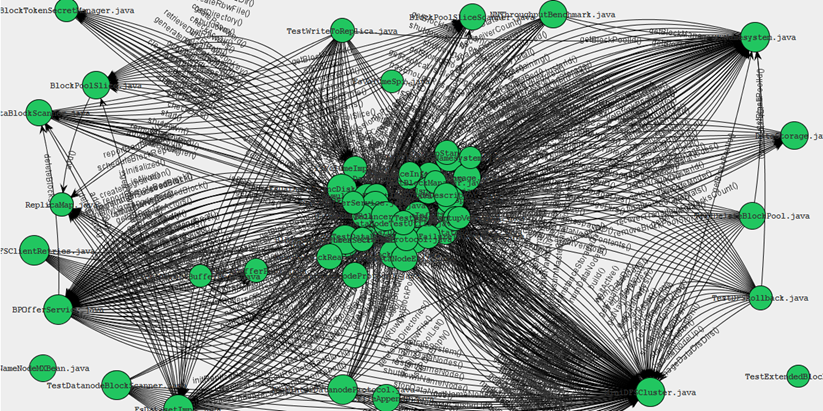
\includegraphics[width=0.99\linewidth]{./img/Pooling}
\caption{Resource Pooling Tactic Implemented in Apache Hadoop Project}
\label{fig:Pooling}
\end{figure}


\subsection{Structure Is Not a Key, But Impacts Code Quality}
Unlike design patterns which tend to be described in terms of classes and their associations, tactics are described in terms of roles and interactions~\cite{bass:arch12}. This means that a tactic is not dependent upon a specific {\em structural} format. While a single tactic might be implemented using a variety of design notions or proprietary designs, the structural properties of tactical files can have a significant impact on the quality of the tactic. Flaws such as cyclic dependencies, improper inheritance, unstable interfaces, and modularity violations are strongly correlated to increased bug rates and the elevated maintenance costs.

Figure~\ref{fig:Pooling} displays the \textit{Resource Pooling} tactic in the Apache Hadoop project. Nodes in this graph represent the source file, and the edges are method calls between the source files. We observed several such tactic implementations that did not expose a well organized code structure. Typically, the source files in the tactic form a full graph with several cyclic dependencies between each pair of files.

\textit{A tactic-search engine should take into account the internal quality of recommended code to avoid suggesting code with design and structural flaws.}


\subsection{Tactical Clones, Right Level of
\\Reuse-Granularity}
While the implementation of tactics vary between different systems, the \textit{intrinsic characteristics of tactics are maintained across different projects}. These are known as \emph{architectural or tactical clones}. Based on our observations, tactical clones are the minimum reusable tactical features. In our code review process, we found that even for a simple tactic like Heartbeat the implementation would result in a large number of interrelated files, with each playing a different role. Some of which include \textit{Heartbeat Emitter}, \textit{Heartbeat Receiver}, \textit{Configuration files} to set Heartbeat intervals and other parameters,\textit{supporting classes and interfaces} to implement each  tactical roles. More complex tactics, specially the cross-cutting ones can easily impact hundreds of source files. Therefore recommending code snippets for those tactics would create a large search space for the developers with lesser degree of reusability.

\textit{The lack of structure, and a concrete micro-level design which can be recovered across multiple projects indicates that method level clones are the right level of granularity.} In the next section we provide examples of such tactical clones.

\subsection{Tactics Are Misused, Degraded or Implemented Incorrectly.} 

Open source repositories contain numerous cases where architectural tactics have been adopted by developers without them fully understanding the driving forces and variability points associated with each tactic and consequences of implementing the tactic~\cite{FSE2012}. The Heartbleed issue is a good example of such a misuse. Heartbeat functionality in OpenSSL is an optional feature, although many developers have ignored this option. %Furthermore, the implementation of heartbeat functionality did not followed solid software engineering practices. DK - Removed this since I felt like it was a weak sentence and would have led to further questions.

In our analysis of bug reports in tactical fragments of the Hadoop project, we found that when a tactical file had a bug, then 89\% of these concerns were due to issues such as unhandled exceptions, type mismatches, or missing values in a configuration file. Incorrect implementations led to 11\% of all reports. These bugs involved misconceptions in the use of the tactic, so that the tactic failed to adequately accomplish its underlying architectural goals. These types of bugs caused the system to crash under certain circumstances. For example, in one case a replication decision with a complex synchronization mechanism was misunderstood for different types of replica failures. Another example was a scheduling tactic which resulted in a deadlock problem. This investigation shows that systems are exposed to new risks during implementation of the tactical decisions.

\textit{A practical tactic search engine, needs to take into account tactical code qualities, and the context in which the tactics are adopted, Additional quality factors include the history of bug fixes and refactoring activities on the candidate clones.}

\subsection{Object Oriented Metrics Are Not Indicator of Tactical Code Quality}
We performed a detailed investigation of bug fixes in two of the systems included in our study. Our initial analysis of the OO metrics of Chidamber et al.\cite{491650} and tactical code snippets in Apache Hadoop and OfBiz indicates that tactical code snippets typically have a relatively higher code complexity compared to non-tactical code snippets~\cite{MSRBuble}. For example, implementing \textit{thread pooling} requires devising solutions for the \textit{thread safe} problem which will results in a more complex implementation. Therefore OO metrics such as \emph{WMC (Weighted Methods per Class)} or~\emph{CBO (Coupling Between Object classes)} can not solely be a good indicator of an improved tactical code snippet.

\textit{A good tactic search engine must take novel code metrics into account to filter potentially complex code samples. Such metrics should help filter code snippets which are difficult to comprehend and modify.}